% !TEX root = ./docs.tex

\author{Jan Grübener, Patrick Mischka}
\subsection{Grafische Oberfläche bei den Nutzern}
<<<<<<< HEAD
Wählt der Nutzer nach dem Starten des Clients die Variante mit Grafischer Benutzeroberfläche starten, ruft der Client die Methode startGui() auf. Hierbei wird ein JFrame erzeugt, auf dem im Laufe der Zeit unterschiedliche JPanels hinzugefügt und entfernt werden. Je nachdem an welchem Punkt der Nutzer sich gerade befindet werden die entsprechenden Methoden wie loginPanel() oder displayRecentConversations() für die jeweilige Funktionalität aufgerufen. \\

//TODO: Erklären: Wie bekommt die GUI neue Chatnachrichten (eigener "Listener" Thread) - passt das so? \\
Bei der Instanziierung des GUI-Objekts wird ebenfalls ein damit referenziertes 
API-Objekt instanziiert. Dieses API-Objekt beinhaltet die Methode 
"startPacketListener". Diese Methode wird bei erfolgreichem login in der GUI 
aufgerufen. Die startPacketListener Methode startet einen Thread, der durchgehend 
einkommende Pakete annimmt, sie überprüft und entsprechende Methodenreferenzen in dem 
GUI-Objekt aufruft. Neue Chats, einkommende Nachrichten und neue Nutzer werden so 
in die GUI übernommen.\\

=======
Wählt der Nutzer nach dem Starten des Clients die Variante mit Grafischer Benutzeroberfläche starten, ruft der Client die Methode startGui() auf. Hierbei wird ein JFrame erzeugt, auf dem im Laufe der Zeit unterschiedliche JPanels hinzugefügt und entfernt werden. Je nachdem an welchem Punkt der Nutzer sich gerade befindet werden die entsprechenden Methoden wie loginPanel() oder displayRecentConversations() für die jeweilige Funktionalität aufgerufen. \\ \\
//TODO: Erklären: Wie bekommt die GUI neue Chatnachrichten (eigener "Listener" Thread) \\
>>>>>>> bc7c57f3cfb482384c7592bfeb8b41ce54e72d32
//TODO (Wenn noch Platz vorhanden): startGui() erklären wie Daten aus Entites gelesen wird
\author{Jan Grübener, Patrick Mischka}
\subsection{Verwendung von Emojis}
Java wandelt den Unicode automatisch in das zugehörige Emoji um, sodass keine Icons für die Emojiauswahl oder weitere Anpassungen im Frontend nötig waren. Bei der Auswahl eines Emojis wird ein Objekt der Klasse EmojiMouseListener instanziiert, welches den entsprechenden Unicode Wert an die JTextArea anhängt. So ist es jederzeit möglich die Anzahl der Emojis zu erhöhen oder Emojis zu tauschen, indem das Gridlayout, welches die Methode renderEmojiPanel() liefert, angepasst wird.

Auf Serverseite mussten hierfür keine Veränderungen vorgenommen werden.

\author{Matthias Vonend, Aaron Schweig, Troy Keßler}
\subsection{Gruppenchats}
Gruppenchats stellen nur eine Erweiterung der bestehenden Chatimplementierung dar. Statt das ein Chat nur die beiden Teilnehmer besitzt, besitzt es nur beliebig viele Nutzer. Wird eine Nachricht empfangen werden nun alle am chatbeteiligten Nutzer durchlaufen und die Nachricht wird an alle der Node bekannten Clients weitergeleitet. Außerdem wird wie bereits erwähnt die Nachricht aus Konsistenzgründen weiter gebroadcastet.

\author{Matthias Vonend, Troy Keßler}
\subsection{Mehrere Chatverläufe pro Nutzer}
Mehrere Chatverläufe sind ähnlich zu den Gruppenchats eine Erweiterung der bestehenden Chatimplementierung. Nun ist es möglich mehrere Chats zu erstellen und zwischen diesen zu wechseln.
//TODO @Troy kannst du hier beschreiben wie das im Client ist (also openChat)

\author{Matthias Vonend}
\subsection{Persistentes Speichern der Chatverläufe}\label{persistance}
Sämtliche der Node bekannten Informationen (Nutzer, Chats, Nachrichten) werden in einem Warehouse verwaltet. Um diese Informationen zwischen Node-Neustarts zu persistieren muss demnach das Warehouse als Datei gespeichert werden und bei Node-Start wieder geladen werden. Existiert noch kein Speicherstand, wird die Node mit einem leeren Warehouse initialisiert.Während die Node ausgefallen ist, können andere Nodes gleichzeitig neue Informationen erhalten haben. Sobald die Node wieder verfügbar ist müssen andere Nodes dies bemerken und die ausgefallene Node mit Informationen versorgen. Um den Ausfall festzustellen ist ein Heart-Beat vorgesehen. Dieser pingt jede Sekunde alle benachbarten Nodes an, um sicherzustellen, dass die Verbindung noch existiert. Sollte eine Unterbrechung festgestellt, versucht die Node die Verbindung wiederaufzubauen. Gelingt dies, so wird das Warehouse übersendet. Jede Node prüft, ob sie alle Informationen des empfangenen Warehouses bereits besitzt und fügt neue Informationen hinzu. Sofern die Node neue Informationen erhalten haben, broadcastet diese ihren neuen Stand an alle benachbarten Nodes um diese auch auf den neuesten Stand zu bringen.

Der Speichervorgang kann je nach System und Warehousegröße längere Zeiten in Anspruch nehmen. In dieser Zeit können in der Regel keine weiteren Anfragen verarbeitet werden. Um diese Zeit zu minimieren kümmert sich ein eigener Thread um die Speicherung und speichert das Warehouse in Intervallen.
Zu beachten ist der Fall, dass eine Node zusammenbricht während der Speichervorgang in Arbeit ist. In diesem Fall würde die Node sämtliche Informationen verlieren, da die Speicherdatei korrupt ist. Um dies zu verhindern wird der Speicherstand zunächst in eine Tempdatei geschrieben und nach erfolgreicher Speicherung an den Zielort verschoben.

\author{Troy Keßler, Michael Angermeier}
\subsection{Verschlüsselte Übertragung der Chat-Nachrichten}\label{encryption}
Um einen sicheren Nachrichtenkanal zu gewährleisten wurde eine Ende-zu-Ende-Verschlüsselung implementiert. Dabei wird beim Erstellen eines Chats unter allen Teilnehmern ein Diffie-Hellman Schlüsselaustausch durchgeführt, sodass jeder Client denselben Schlüssel für einen Chat besitzt. Diese generierten Schlüssel werden beim Client zur Chat ID lokal gespeichert, sodass der auch nach einem Neustart weiter den Chat nutzen kann. Somit kann der Client, bevor er Nachrichten zum Server sendet, den Inhalt mit dem jeweiligen Chat Schlüssel verschlüsseln und ankommende Nachrichten entschlüsseln. Somit wird der Server ausschließlich verschlüsselte Nachrichten erhalten, auf die er keinen Zugriff hat.

Die öffentlichen Schlüssel wurden dabei für jeden Client festgeschrieben. Nach jedem Login und nach Erstellen eines Chats generiert der Client einen neuen 128bit Schlüssel und löscht den alten, um die Sicherheit zu erhöhen. Um auch Gruppenchats ermöglichen zu können musste der Diffie-Hellman-Schlüsselaustausch entsprechend erweitert werden. Dabei gibt es in Gruppen im Gegensatz zu zwei Teilnehmern mehrere Runden. Ein Schlüsselaustausch mit drei Teilnehmern kann aus Abbildung 2 entnommen werden.

\begin{figure}[h]
  \centering
  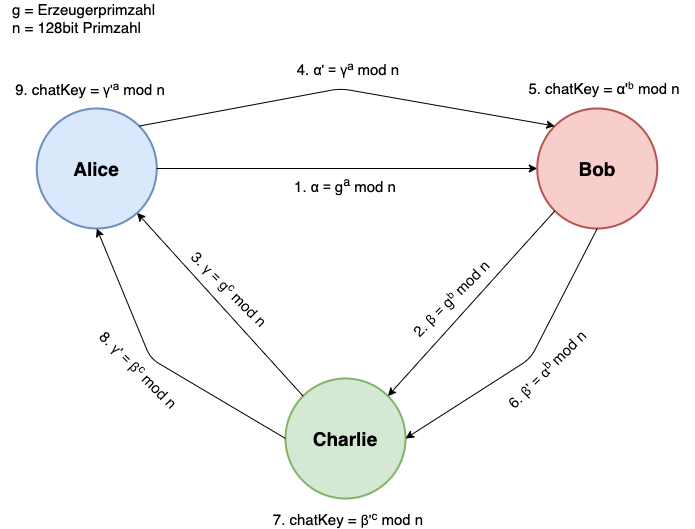
\includegraphics[width=\textwidth]{dh.png}
  
  \caption{Erweiterter Diffie-Hellman}
\end{figure}

Wie man erkennen kann werden in der ersten Runde (Schritte 1-3) die ersten Teilschlüssel wie im klassischen Diffie-Hellman generiert und weitergeschickt. In der zweiten Runde wird mithilfe der Ergebnisse der ersten Runde, die fertigen Chat Schlüssel berechnet (Schritte 4-9). Die Größe der Primzahl n beträgt 128bit, wobei die Länge der Generatorprimzahl 32bit ist. Somit ergibt sich für den Chat ein Schlüssel von ebenfalls 128bit.

\newpage

Dieses Verfahren kann mit beliebig vielen Teilnehmern durchgeführt
werden, jedoch steigt die Anzahl der Runden linear und die Anzahl der 
Requests quadratisch.

$$ rounds = n - 1 $$
$$ requests = n \cdot (n - 1) $$

Wobei hier n die Anzahl der Teilnehmer ist.

Aus Implementierungssicht braucht der Initiator dieses
Schlüsselaustauschs eine Endbedingung, sodass er nachdem
die Schlüssel unter allen Teilnehmern ausgetauscht wurden 
den Chat erstellen kann. Der Initiator dieses Schlüsselaustauschs 
kann nun mit dem Bedingung

$$ currentRequests = (targetRequests - userIndex) $$

prüfen, ob der Schlüsselaustausch vollständig durchgeführt wurde. Dabei steht 
$ currentRequests $ für die Anzahl, wie oft das Paket schon weitergeleitet
wurde. Diese wird beim versenden inkrementiert. $ targetRequests $
ist die Anzahl der theoretischen Requests die gesendet werden müssen, diese
beträgt wie oben definiert immer $ n \cdot (n - 1) $. $ userIndex $ steht
für die Position im Schlüsselaustausch, der Initiator ist der Erste, sodass
dieser bei ihm 0 ist. Im obigen Beispiel wäre also die Endbedingung
erfüllt wenn der Initiator ein Paket erhält, welches schon sechs mal 
weitergeleitet wurde.

$$ 6 = (3 * (3 - 1)) - 0 $$

Für alle anderen Clients gilt eine leicht abgeänderte Endbedingung.

Da nun alle Chatteilnehmer den gleichen Schlüssel besitzen, dieser 
lokal gesichert, und der Chat erstellt ist können Nachrichten mit 
einem symmetrischen Verfahren sicher versendet werden. Für dieses 
symmetrische Verfahren wurde die AES Verschlüsselung gewählt und
implementiert.

\author{Troy Keßler}
\subsection{Verschlüsselte serverseitige Speicherung der Chats}
Durch die in \ref{encryption} beschriebene Ende-zu-Ende Verschlüsselung liegen dem Server die Nachrichten nie in Klartextform vor, sondern stets in der verschlüsselten Form. Wie bereits in \ref{persistance} erwähnt werden alle Nachrichten im Warehouse gespeichert und das gesamte Warehouse wird abgespeichert. So liegen auch in der Speicherdatei die Nachrichten niemals in Klartextform vor.
